% High-level system design. Compile with Tectonic or XeLaTeX.
% This file is editable. Regenerate from Markdown only with --from-markdown.
\documentclass[12pt,letterpaper]{article}
\usepackage[margin=0.8in]{geometry}
\usepackage{fontspec}
\IfFileExists{/System/Library/Fonts/Supplemental/Times New Roman.ttf}{%
  \setmainfont{Times New Roman}[Path=/System/Library/Fonts/Supplemental/,
    Extension=.ttf,UprightFont=*,BoldFont=* Bold,ItalicFont=* Italic,
    BoldItalicFont=* Bold Italic]
}{\setmainfont{Times New Roman}}
\IfFileExists{/System/Library/Fonts/Supplemental/Times New Roman.ttf}{%
  \setmonofont{Times New Roman}[Path=/System/Library/Fonts/Supplemental/,Extension=.ttf]
}{\setmonofont{Times New Roman}}
\usepackage{graphicx}
\usepackage{booktabs,longtable,array,ragged2e}
\usepackage{fancyvrb}
\usepackage{caption}
\usepackage[hidelinks]{hyperref}
\hypersetup{pdftitle={In-Home Assistive Robot: High-Level System Design},
  pdfauthor={Gavin Lamphier; Liam Patel; Austin Heiss}}
\captionsetup{font=small,labelfont=bf,labelsep=period,skip=8pt,hypcap=false}
\setlength{\parindent}{0pt}
\setlength{\parskip}{6pt plus 1pt}
\setlength{\emergencystretch}{2em}
\setlength{\LTpre}{8pt}
\setlength{\LTpost}{10pt}
\renewcommand{\baselinestretch}{1.08}
\newcommand{\schema}[1]{{\normalfont #1}}
\pagestyle{plain}
\begin{document}


\begin{titlepage}

\centering

\vspace*{1.2in}

{\LARGE\bfseries In-Home Assistive Robot\par}

\vspace{0.25in}

{\Large High-Level System Design\par}

\vspace{0.12in}

{\large Design D0\par}

\vspace{0.8in}

\begin{tabular}{ll}

Gavin Lamphier & Industrial Design \\[6pt]

Liam Patel & Mechanical Engineering \\[6pt]

Austin Heiss & Computer Science \\[6pt]

\end{tabular}

\vspace{0.55in}

\par October 2, 2026

\vfill

\begin{minipage}{0.84\textwidth}

\textbf{Goal.} Our robot lets an older or disabled adult at home take video calls from a family caregiver and, if they want, have the robot follow them from room to room during the call. The robot stops following as soon as it loses track of them or a safety check fails.

\end{minipage}

\par\vspace{0.16in}{\small AI was used to format this document in \LaTeX.\par}

\vspace*{0.6in}

\end{titlepage}

\setcounter{page}{1}

\section{Title, goal statement, and conventions}

\textbf{Goal:} Our robot lets an older or disabled adult at home take video calls from a family caregiver and, if they want, have the robot follow them from room to room during the call. The robot stops following as soon as it loses track of them or a safety check fails.

The basic input to the system is a caregiver's call request, the resident's choices, and readings from the robot's sensors. The basic output is a two-way video call that the resident has accepted, a clear display of the call and privacy status, and robot movement that either follows the resident or stops.

We are designing and building the robot's physical platform ourselves (the chassis, mounts, enclosure, and mechanisms) and fitting it with purchased motors, sensors, electronics, and a screen. For this first design we are focusing on calls and on following the resident when they ask, in a controlled, single-floor indoor space. We have also talked about item delivery, reminders, an adjustable screen, and help detection, but have not decided on those yet.

In each diagram, blue rounded boxes are parts we build and gray dashed boxes are outside services we rely on. Stick figures are people, and dashed blue outlines show where the software runs. Arrows point in the direction information or control moves, and the I1-I16 labels match the rows of the interface table. The red line is the planned direct wire for the Stop and Privacy buttons, and the small open-ended boxes are places where information is stored.

Every part traces back to at least one of our five user stories. Keeping a call going while the resident moves (US-01) uses the whole system. The resident controls and the call manager make sure nothing starts without the resident's consent (US-02). The call server and caregiver app tell the caregiver what happened to a call (US-03). Person tracking, motion control, and the platform keep the robot from following the wrong person (US-04). The resident controls, and where we place them, make the robot usable from a seat (US-05).

\section{Block diagram (the D0 diagram)}

\begin{center}
\begin{minipage}{\linewidth}
\centering
\makebox[\linewidth]{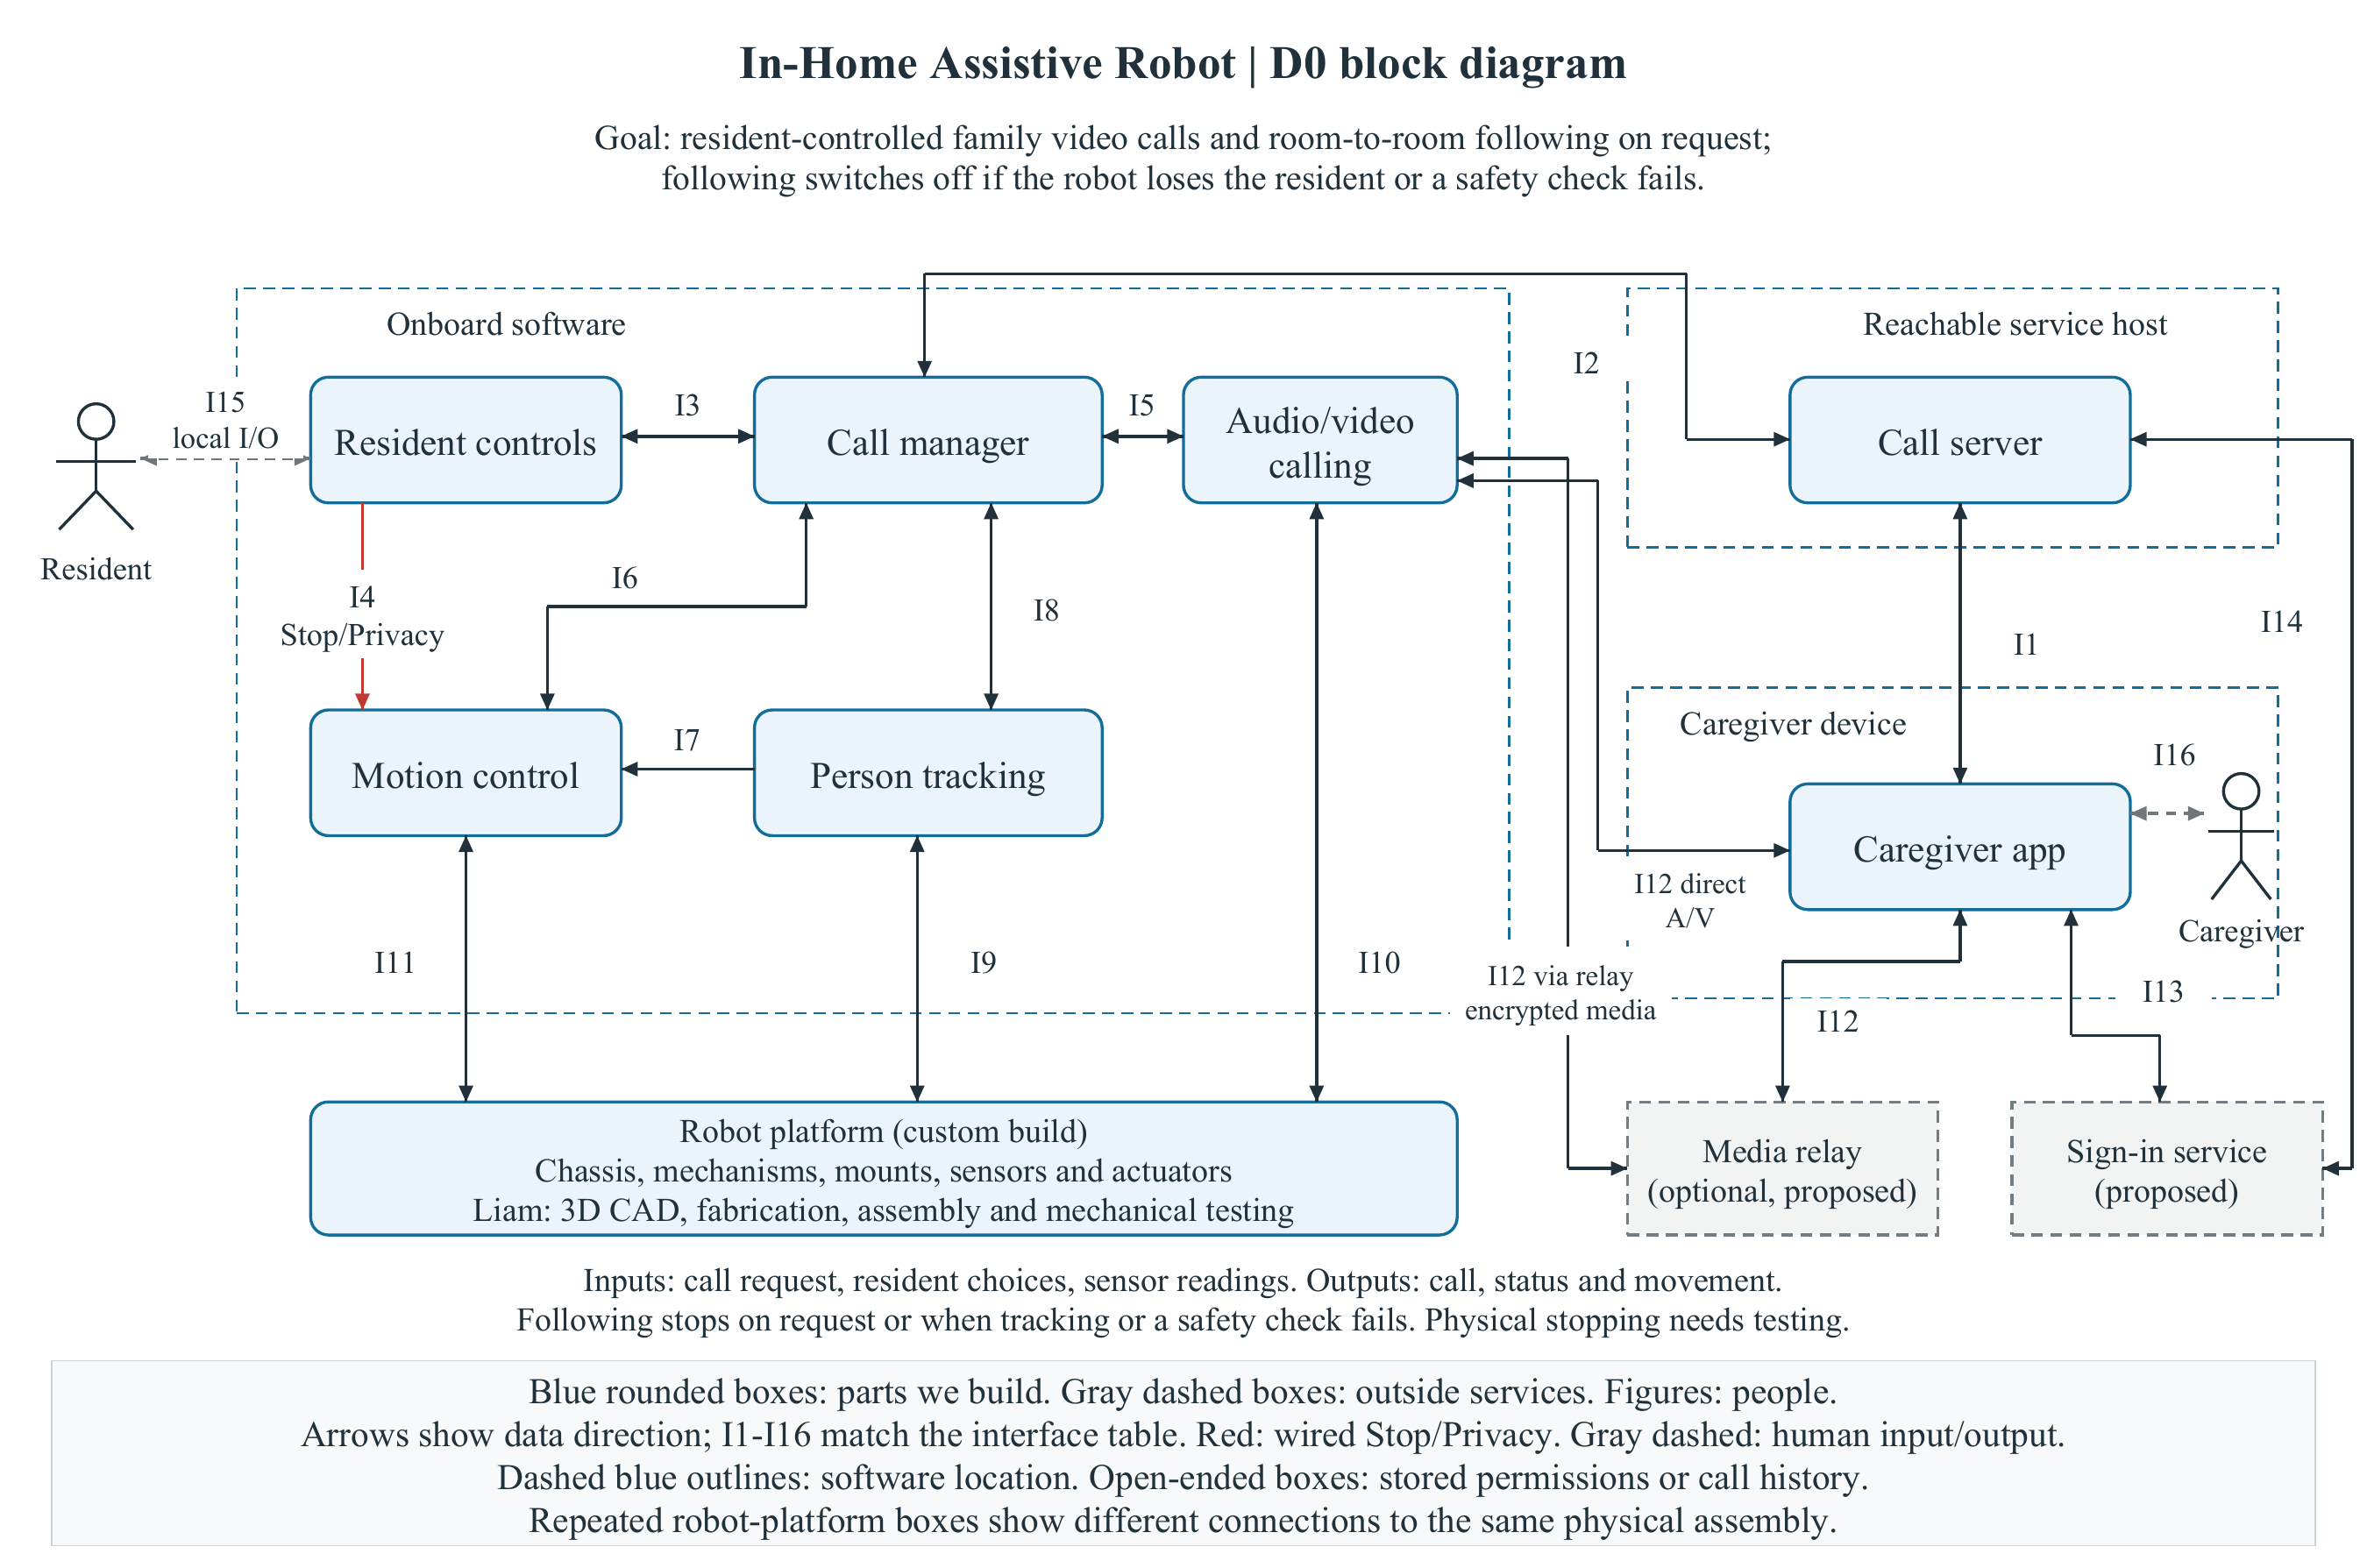
\includegraphics[width=1.08\linewidth,height=0.6\textheight,keepaspectratio]{D0_block_diagram.png}}
\captionof{figure}{System block diagram}\label{fig:1}
\end{minipage}
\end{center}

The robot's software runs on the platform we are building, while the call server and caregiver app run separately. We plan to use an outside sign-in service and, when a direct connection fails, a media relay, but we have not picked providers for either yet.

\section{Component responsibility table}

Liam is in charge of the mechanical build: 3D modeling, chassis and mechanism design, fabrication, assembly, and mechanical testing. He will also plan test fixtures and check fit, strength, clearances, and low-speed driving. Gavin is in charge of the robot's form, where the screen and controls go, and the experience for both the resident and the caregiver. Austin is in charge of the software, communication, sensing, and control code, and works with Liam where the mechanical and electrical parts meet.

\begingroup
\small
\setlength{\tabcolsep}{5pt}
\renewcommand{\arraystretch}{1.12}
\begin{longtable}{@{}>{\RaggedRight\arraybackslash}p{\dimexpr 0.47\linewidth-2\tabcolsep\relax}>{\RaggedRight\arraybackslash}p{\dimexpr 0.25\linewidth-2\tabcolsep\relax}>{\RaggedRight\arraybackslash}p{\dimexpr 0.28\linewidth-2\tabcolsep\relax}@{}}
\caption{Responsibilities for the eight parts of the system}\label{tab:components}\\
\toprule
\textbf{Component and responsibility} & \textbf{Interfaces} & \textbf{Owner and stories} \\
\midrule
\endfirsthead
\caption[]{Responsibilities for the eight parts of the system}\\
\toprule
\textbf{Component and responsibility} & \textbf{Interfaces} & \textbf{Owner and stories} \\
\midrule
\endhead
\midrule
\endfoot
\bottomrule
\endlastfoot
Resident controls: Gives the resident the screen and buttons for calls, privacy, and following. & In: I3, I15. Out: I3, I4, I15 & Gavin Lamphier. US-01, US-02, US-04, US-05 \\ \addlinespace[3pt]
Call manager: Decides what the call and the robot are allowed to do, based on the resident's choices. & In: I2, I3, I5, I6, I8. Out: I2, I3, I5, I6, I8 & Austin Heiss. US-01, US-02, US-03, US-04, US-05 \\ \addlinespace[3pt]
Audio/video calling: Sends and receives live audio and video once the resident accepts a call. & In: I5, I10, I12. Out: I5, I10, I12 & Austin Heiss. US-01, US-02, US-03, US-05 \\ \addlinespace[3pt]
Person tracking: Reports where the selected resident is, or that it can't find them. & In: I8, I9. Out: I7, I8, I9 & Austin Heiss. US-01, US-02, US-04, US-05 \\ \addlinespace[3pt]
Motion control: Turns the resident's position into movement commands, requesting a stop whenever it should. & In: I4, I6, I7, I11. Out: I6, I11 & Liam Patel. US-01, US-04, US-05 \\ \addlinespace[3pt]
Robot platform: Is the physical robot that carries the sensors, screen, speaker, and motors. & In: I9, I10, I11. Out: I9, I10, I11 & Liam Patel. US-01, US-04, US-05 \\ \addlinespace[3pt]
Call server: Keeps track of each call attempt so the caregiver and the robot agree on its status. & In: I1, I2, I14. Out: I1, I2, I14 & Austin Heiss. US-01, US-02, US-03 \\ \addlinespace[3pt]
Caregiver app: Lets the caregiver start or end a call and see what happened to it. & In: I1, I12, I13, I16. Out: I1, I12, I13, I16 & Gavin Lamphier. US-01, US-03 \\*
\end{longtable}
\endgroup

\section{Interface specification table}

Each row lists the main fields and their types, the data format, how the data is sent, and which part handles a failure. We plan for the parts on the robot to talk through function calls inside one program; we still need to choose the physical connections and the outside service providers. A call's status is one of ringing, connected, declined, no answer, offline, ended, or failed.

\begingroup\small
\setlength{\tabcolsep}{5pt}
\renewcommand{\arraystretch}{1.12}
\begin{longtable}{@{}>{\RaggedRight\arraybackslash}p{0.21\linewidth}>{\RaggedRight\arraybackslash}p{\dimexpr 0.79\linewidth-2\tabcolsep\relax}@{}}
\caption{Interface specifications}\label{tab:interfaces}\\
\toprule\textbf{Connection} & \textbf{Specification}\\\midrule\endfirsthead
\caption[]{Interface specifications}\\
\toprule\textbf{Connection} & \textbf{Specification}\\\midrule\endhead
\midrule\endfoot
\bottomrule\endlastfoot
I1 caregiver app <-> call server & \textbf{Inputs and outputs.} Request: \schema{robot\_\allowbreak{}id} and \schema{access\_\allowbreak{}token} (text), \schema{action} (start or end). Response: \schema{call\_\allowbreak{}id} (text), \schema{status} (call status), \schema{last\_\allowbreak{}seen} (timestamp or none).\par\smallskip \textbf{Data format.} JSON\par\smallskip \textbf{Protocol.} HTTPS requests; secure WebSocket status updates\par\smallskip \textbf{Error behavior and handler.} The call server rejects bad requests, and the app tells the caregiver when it can't connect. \\ \addlinespace[4pt]
I2 call server <-> call manager & \textbf{Inputs and outputs.} Invitation: \schema{call\_\allowbreak{}id} and \schema{caller\_\allowbreak{}name} (text). Response: \schema{call\_\allowbreak{}id} (text), \schema{status} (call status); \schema{robot\_\allowbreak{}online} (boolean).\par\smallskip \textbf{Data format.} JSON\par\smallskip \textbf{Protocol.} Secure WebSocket; robot sends status each second\par\smallskip \textbf{Error behavior and handler.} The server reports the robot offline after 5 seconds without an update; if the connection drops during a call, the call manager ends the call. \\ \addlinespace[4pt]
I3 resident controls <-> call manager & \textbf{Inputs and outputs.} Input: \schema{action} (accept, decline, end, follow, stop, or privacy), \schema{target\_\allowbreak{}id} (text or none). Output: \schema{caller\_\allowbreak{}name} (text), \schema{call\_\allowbreak{}status} and \schema{follow\_\allowbreak{}status} (status).\par\smallskip \textbf{Data format.} Typed in-memory records\par\smallskip \textbf{Protocol.} Proposed in-process request and status calls\par\smallskip \textbf{Error behavior and handler.} The call manager ignores actions that don't make sense at that moment, and the controls show an error. \\ \addlinespace[4pt]
I4 resident controls -> motion control & \textbf{Inputs and outputs.} Input: \schema{stop} and \schema{privacy} (on/off). Status returns on I6 and I3.\par\smallskip \textbf{Data format.} Digital signal\par\smallskip \textbf{Protocol.} Proposed direct wired contacts\par\smallskip \textbf{Error behavior and handler.} Motion control requests a stop when Stop or Privacy is pressed, or if the wire is broken. \\ \addlinespace[4pt]
I5 call manager <-> audio/video calling & \textbf{Inputs and outputs.} Input: \schema{capture\_\allowbreak{}allowed} (boolean). Output: \schema{media\_\allowbreak{}status} (connecting, connected, or failed).\par\smallskip \textbf{Data format.} Typed in-memory records\par\smallskip \textbf{Protocol.} Proposed in-process permission and status calls\par\smallskip \textbf{Error behavior and handler.} Audio/video calling stops capture if permission is lost; the call manager reports failure. \\ \addlinespace[4pt]
I6 call manager <-> motion control & \textbf{Inputs and outputs.} Input: \schema{follow\_\allowbreak{}requested} (boolean). Output: \schema{motion\_\allowbreak{}status} (following, stopping, stopped, or fault).\par\smallskip \textbf{Data format.} Typed in-memory records\par\smallskip \textbf{Protocol.} Proposed in-process request and status calls\par\smallskip \textbf{Error behavior and handler.} Motion control requests a stop if following is no longer allowed or requested, and the call manager shows the new status. \\ \addlinespace[4pt]
I7 person tracking -> motion control & \textbf{Inputs and outputs.} Output: \schema{target\_\allowbreak{}id} (text), \schema{range\_\allowbreak{}m} and \schema{bearing\_\allowbreak{}deg} (numbers or none), \schema{tracking\_\allowbreak{}status} (valid or unavailable).\par\smallskip \textbf{Data format.} Typed in-memory record\par\smallskip \textbf{Protocol.} Proposed in-process position update\par\smallskip \textbf{Error behavior and handler.} Motion control requests a stop if tracking becomes unavailable, then waits until the resident asks it to follow again. \\ \addlinespace[4pt]
I8 call manager <-> person tracking & \textbf{Inputs and outputs.} Input: \schema{tracking\_\allowbreak{}allowed} (boolean), \schema{target\_\allowbreak{}id} (text). Output: \schema{tracking\_\allowbreak{}status} (valid or unavailable).\par\smallskip \textbf{Data format.} Typed in-memory records\par\smallskip \textbf{Protocol.} Proposed in-process permission and status calls\par\smallskip \textbf{Error behavior and handler.} If tracking is no longer allowed, person tracking stops and reports itself as unavailable. \\ \addlinespace[4pt]
I9 robot platform <-> person tracking & \textbf{Inputs and outputs.} Input: \schema{capture\_\allowbreak{}requested} (boolean). Output: \schema{image} (image frame), \schema{distance\_\allowbreak{}m} (numbers), \schema{sensor\_\allowbreak{}status} (available or unavailable).\par\smallskip \textbf{Data format.} Image and numeric sensor data\par\smallskip \textbf{Protocol.} Local sensor-driver calls; physical connections to be selected\par\smallskip \textbf{Error behavior and handler.} If the sensors aren't working, person tracking reports them as unavailable and doesn't give a position. \\ \addlinespace[4pt]
I10 robot platform <-> audio/video calling & \textbf{Inputs and outputs.} Input: \schema{camera\_\allowbreak{}frame} (image), \schema{mic\_\allowbreak{}audio} (audio). Output: \schema{display\_\allowbreak{}frame} (image), \schema{speaker\_\allowbreak{}audio} (audio), \schema{capture\_\allowbreak{}requested} (boolean).\par\smallskip \textbf{Data format.} Image and audio buffers; typed control record\par\smallskip \textbf{Protocol.} Local camera, audio, and display driver calls; physical connections to be selected\par\smallskip \textbf{Error behavior and handler.} If the camera, microphone, speaker, or display fails, audio/video calling reports it and ends the call. \\ \addlinespace[4pt]
I11 motion control <-> robot platform & \textbf{Inputs and outputs.} Output: \schema{speed\_\allowbreak{}m\_\allowbreak{}s} and \schema{turn\_\allowbreak{}rate\_\allowbreak{}deg\_\allowbreak{}s} (numbers). Input: \schema{measured\_\allowbreak{}speed\_\allowbreak{}m\_\allowbreak{}s} (number), \schema{path\_\allowbreak{}clear} (boolean), \schema{platform\_\allowbreak{}status} (available or fault).\par\smallskip \textbf{Data format.} Numeric control and sensor records\par\smallskip \textbf{Protocol.} Local motor and sensor driver calls; physical connections to be selected\par\smallskip \textbf{Error behavior and handler.} Motion control requests a stop if sensor feedback stops arriving. We still need to test how well the robot actually stops. \\ \addlinespace[4pt]
I12 audio/video calling <-> caregiver app; optional media relay & \textbf{Inputs and outputs.} Both directions: \schema{video} (video stream), \schema{audio} (audio stream).\par\smallskip \textbf{Data format.} Encoded audio/video packets\par\smallskip \textbf{Protocol.} Proposed encrypted WebRTC, directly or through a relay\par\smallskip \textbf{Error behavior and handler.} Audio/video calling reports when the connection is lost, and the caregiver app shows that the call failed. \\ \addlinespace[4pt]
I13 caregiver app <-> sign-in service & \textbf{Inputs and outputs.} Input: \schema{sign\_\allowbreak{}in} (credential text). Output: \schema{authenticated} (boolean), \schema{access\_\allowbreak{}token} (text).\par\smallskip \textbf{Data format.} Sign-in form and JSON response\par\smallskip \textbf{Protocol.} HTTPS\par\smallskip \textbf{Error behavior and handler.} The caregiver app shows that sign-in failed and won't place calls until the caregiver signs in. \\ \addlinespace[4pt]
I14 call server <-> sign-in service & \textbf{Inputs and outputs.} Input: \schema{access\_\allowbreak{}token} (text). Output: \schema{valid} (boolean), \schema{caregiver\_\allowbreak{}id} (text).\par\smallskip \textbf{Data format.} JSON\par\smallskip \textbf{Protocol.} HTTPS verification request\par\smallskip \textbf{Error behavior and handler.} If the call server can't verify a request, it rejects it and reports a service error. \\ \addlinespace[4pt]
I15 resident <-> resident controls & \textbf{Inputs and outputs.} Input: \schema{action} (touch/button choice). Output: \schema{caller\_\allowbreak{}name} (text), \schema{privacy}, \schema{following}, \schema{camera}, and \schema{microphone} (on, off, or unknown), \schema{alert} (sound).\par\smallskip \textbf{Data format.} Touch/button events; text, indicators, and sound\par\smallskip \textbf{Protocol.} Local button and screen interaction\par\smallskip \textbf{Error behavior and handler.} Resident controls show an error if an action cannot be completed. \\ \addlinespace[4pt]
I16 caregiver <-> caregiver app & \textbf{Inputs and outputs.} Input: \schema{action} (call or end). Output: \schema{call\_\allowbreak{}status} (call status), \schema{video} (video stream), \schema{audio} (audio stream).\par\smallskip \textbf{Data format.} Touch/click events; text and audio/video\par\smallskip \textbf{Protocol.} Phone or browser interaction\par\smallskip \textbf{Error behavior and handler.} The caregiver app displays an unavailable or failed status when a call cannot connect. \\ \addlinespace[4pt]
\end{longtable}
\endgroup

For example, a caregiver starting a call on I1 would send the robot's ID, their sign-in token, and the action:

\begin{quote}
\begin{Verbatim}[fontfamily=tt,fontsize=\small]

{"robot_id": "home-robot-01", "access_token": "example", "action": "start"}

\end{Verbatim}
\end{quote}

\par\ifdim\dimexpr\pagegoal-\pagetotal\relax<1.5in\newpage\fi

\section{Data-flow diagram}

In the call flow, the caregiver's request goes through the call server to the robot. The resident sees who is calling and decides whether to answer. Once they accept, live audio and video go between the robot and the caregiver, and the call status comes back through the server. In this first design, the camera and microphone are only used during a call the resident has accepted.

\begin{center}
\begin{minipage}{\linewidth}
\centering
\makebox[\linewidth]{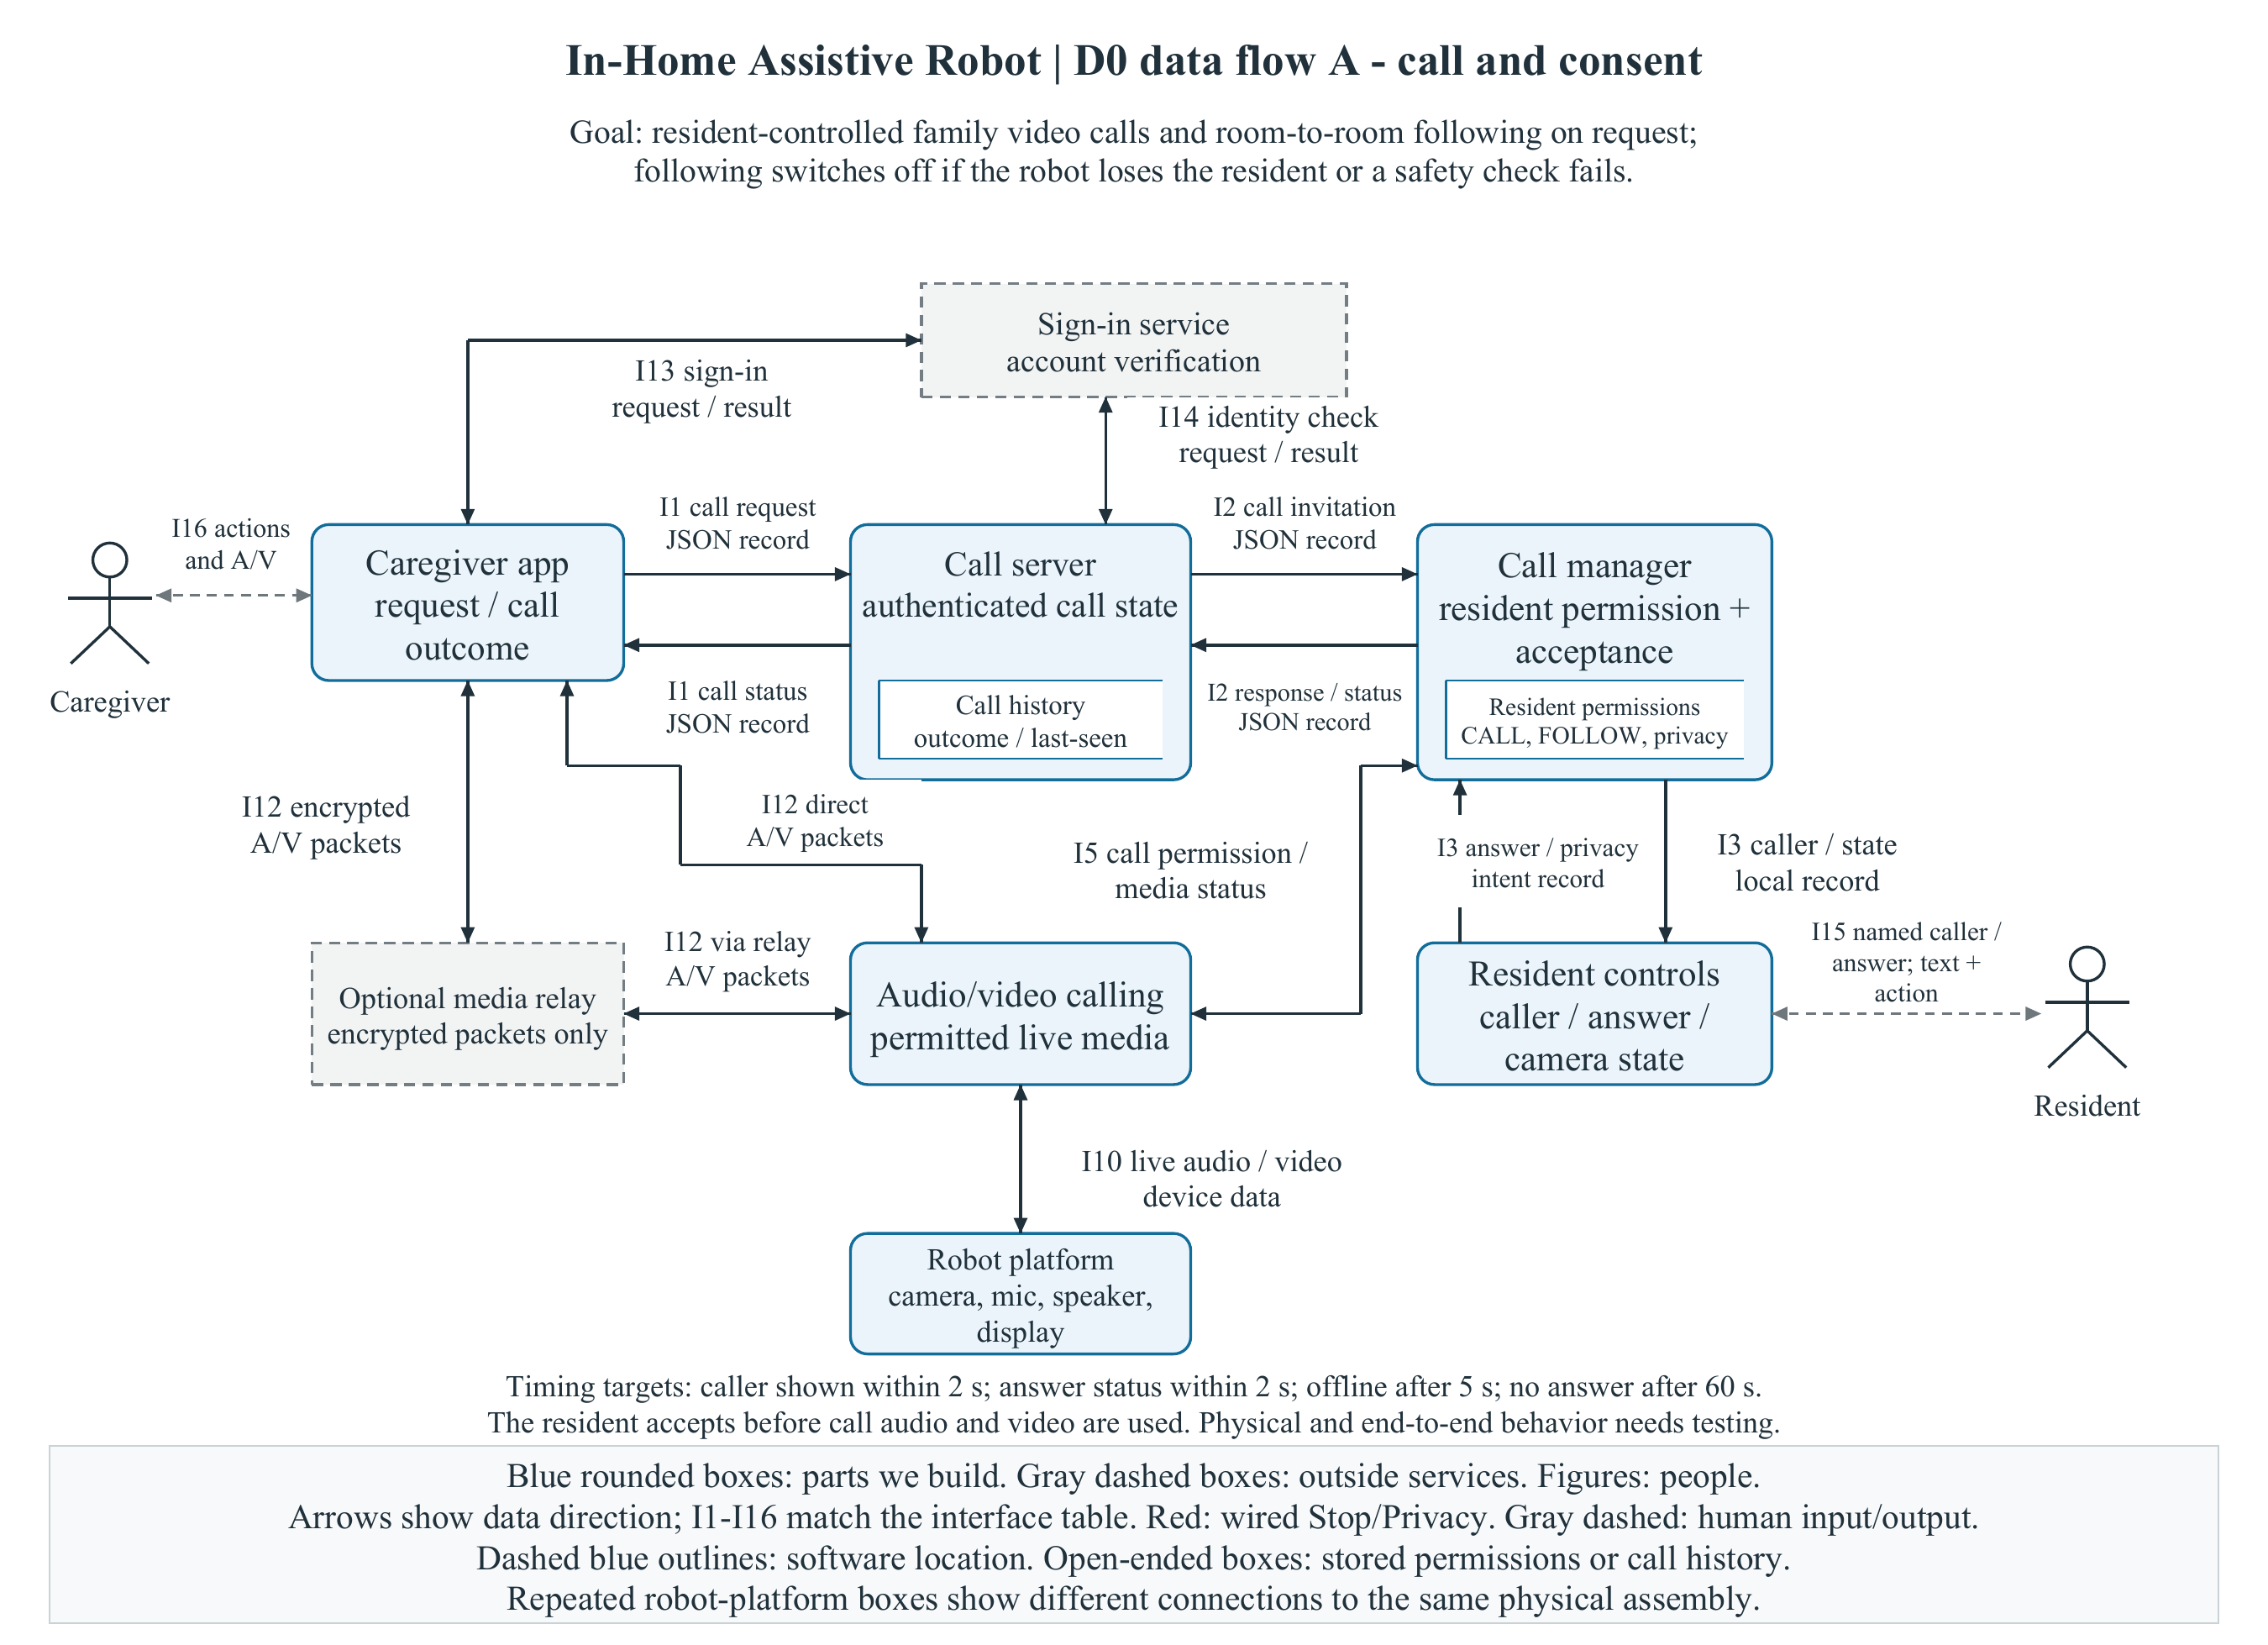
\includegraphics[width=1.08\linewidth,height=0.6\textheight,keepaspectratio]{D0_data_flow_A_call.png}}
\captionof{figure}{Call and consent data flow}\label{fig:2}
\end{minipage}
\end{center}

In the following flow, the resident asks the robot to follow them. The robot's sensor readings are turned into the selected person's position, and motion control uses that position along with the robot's safety checks to decide how to move. If the robot loses the person, the resident turns following off, or a safety check fails, motion control requests a stop. After losing the person, the robot won't start following again until the resident asks, but the call can keep going while the robot is stopped. We still have to test how well the robot actually stops once it is built.

\begin{center}
\begin{minipage}{\linewidth}
\centering
\makebox[\linewidth]{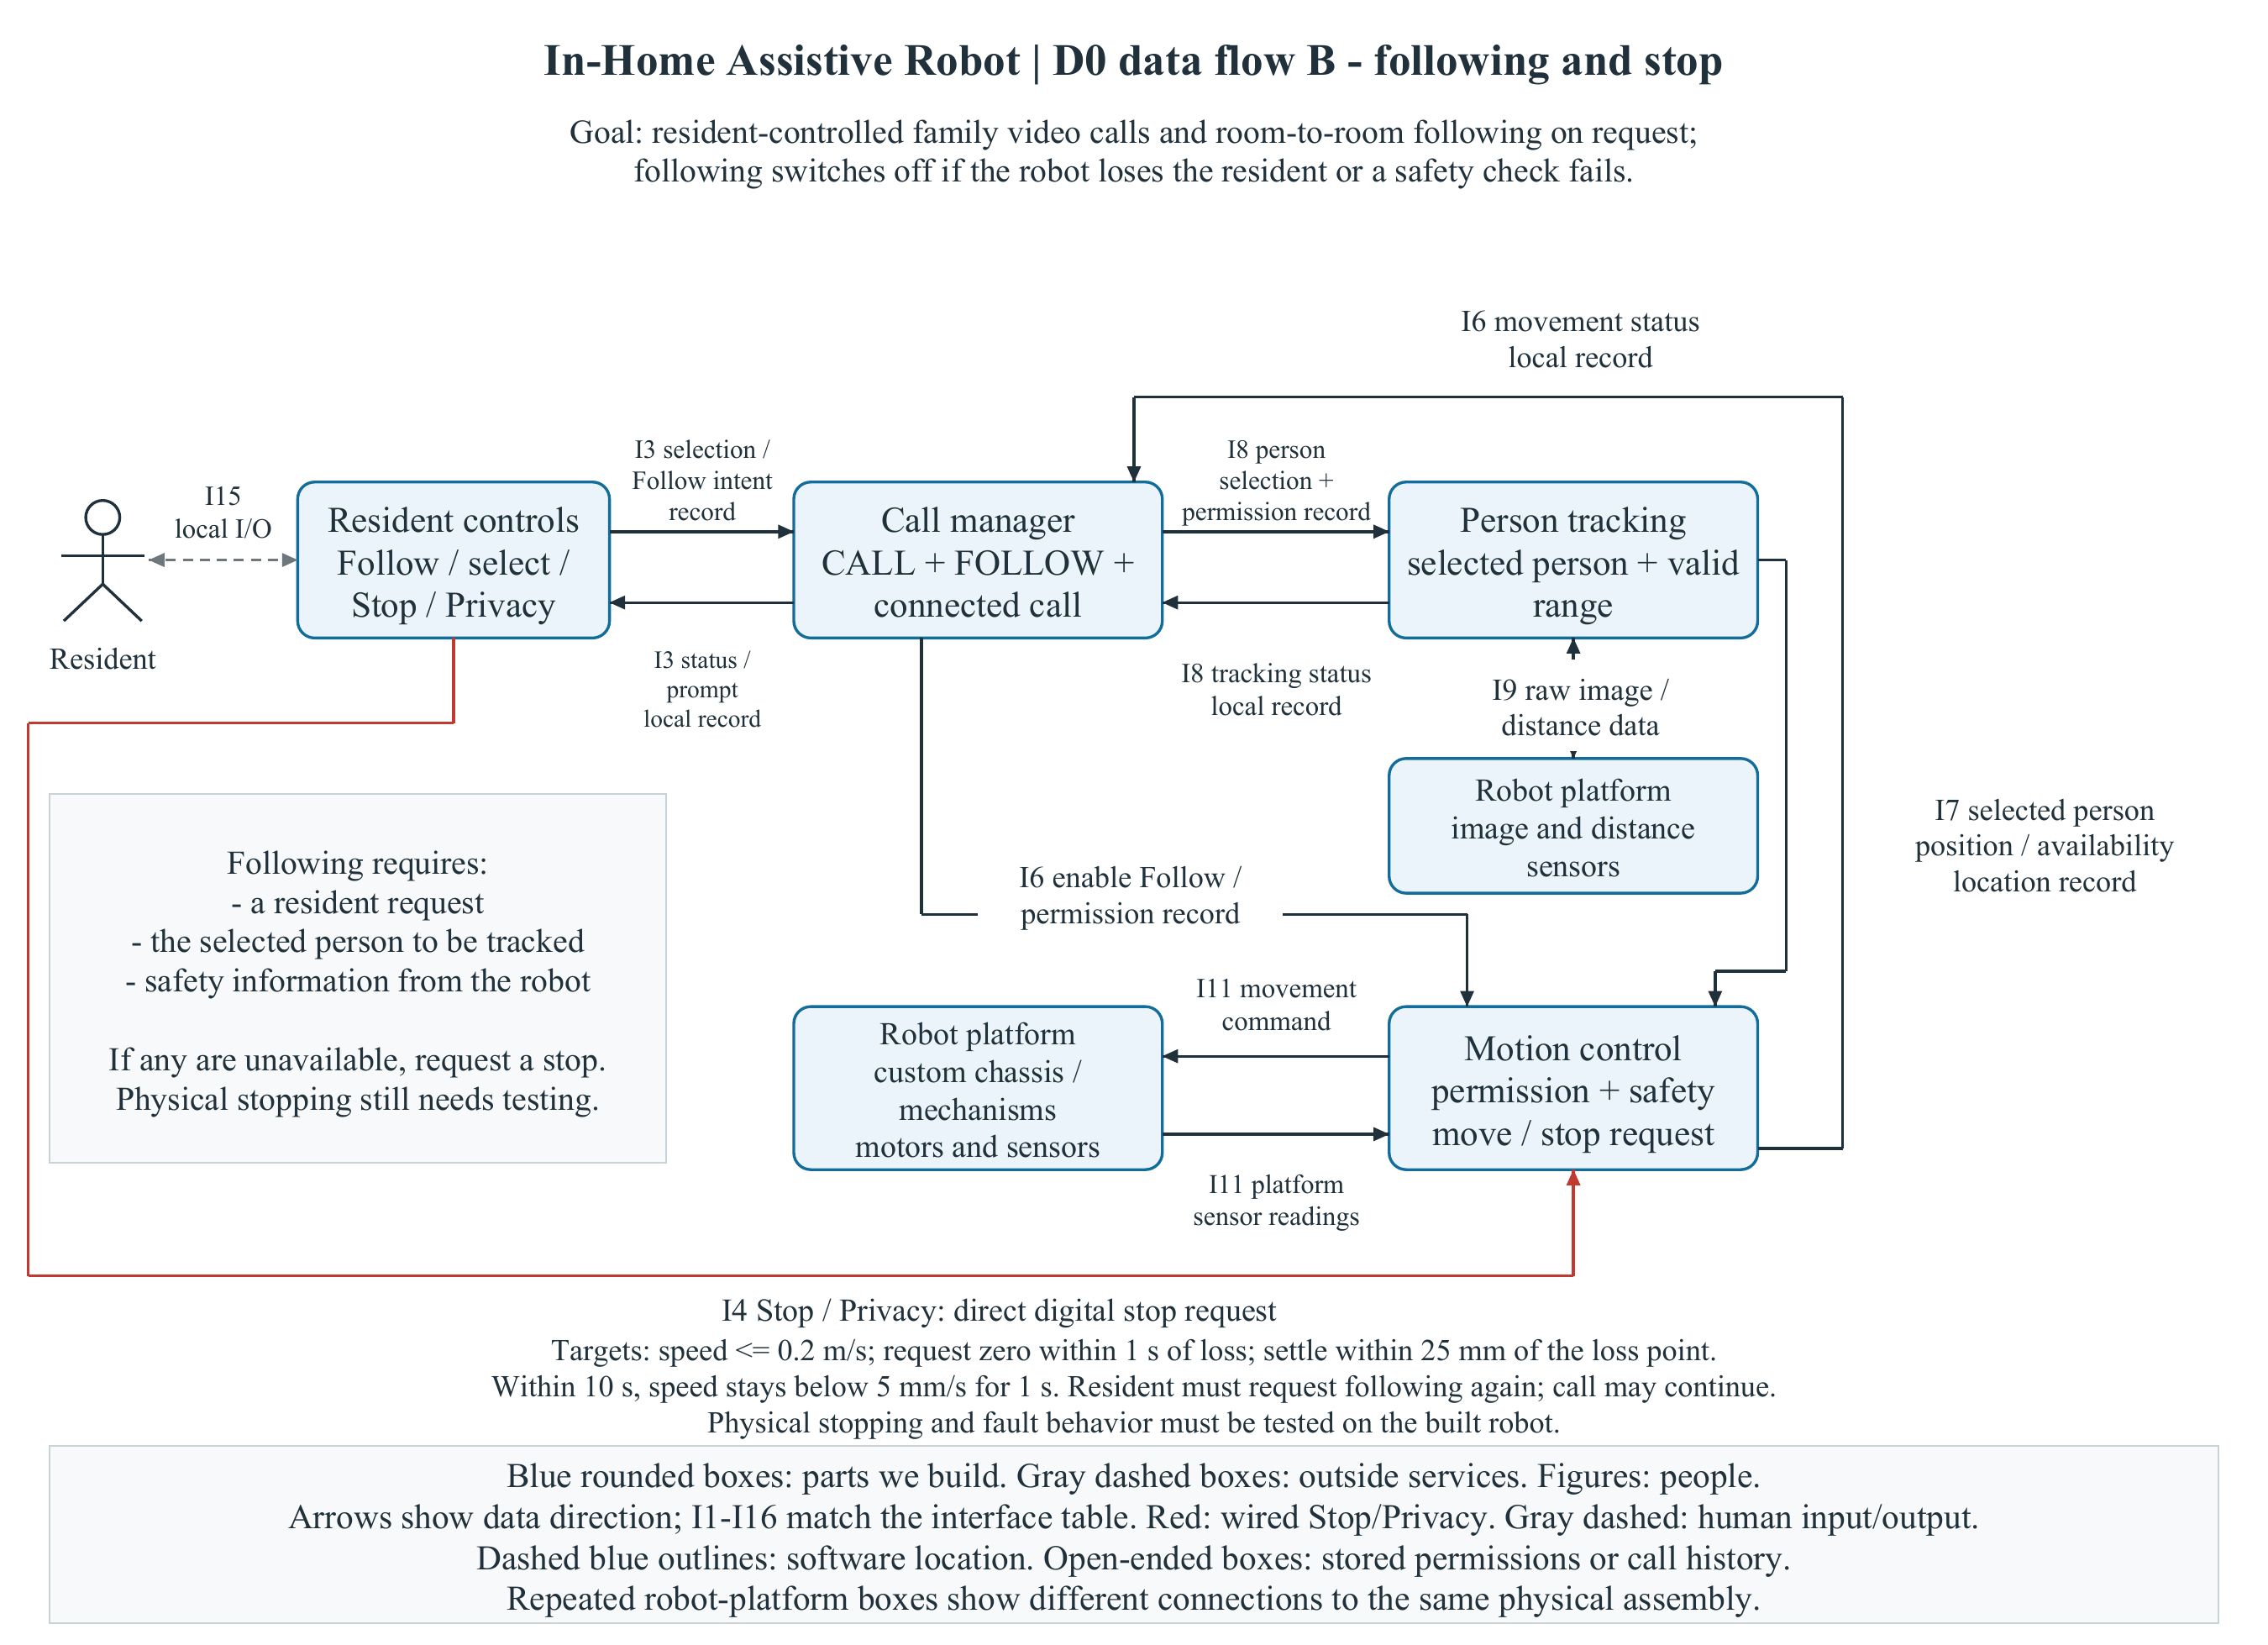
\includegraphics[width=1.08\linewidth,height=0.6\textheight,keepaspectratio]{D0_data_flow_B_follow.png}}
\captionof{figure}{Following and stop data flow}\label{fig:3}
\end{minipage}
\end{center}

Our user stories set a maximum following speed of 0.2 m/s and require the movement request to drop to zero within 1 second of losing the person. After that, the robot has to settle within 25 mm of where it lost the resident and stay below 5 mm/s for a full second, all within 10 seconds. These are targets for the design; we haven't shown them on the physical robot yet.

\section{Architecture pattern and justification}

We use a \textbf{client-server} pattern for communication: the caregiver app and the robot both connect to a call server that keeps track of each call's status. On the robot, a \textbf{layered} design separates the resident controls, the call manager, and the services underneath that handle communication and movement. Following works as a \textbf{pipeline} that goes from sensor readings to a position estimate to a movement command. Finally, the motion hardware follows an \textbf{embedded sensor-actuator} pattern so that movement control stays on the robot.

\textbf{Fit to the problem.} Our project combines remote communication with a physical robot, so we need a server for the communication side and local control for the robot side. These four patterns cover both.

\textbf{Team skills.} The split matches what each of us is good at: Gavin leads interaction design, Liam leads the mechanical build and testing, and Austin leads software and sensing.

\textbf{Performance and timing.} The robot has to react to a lost person or a Stop press even if the internet goes down, so movement and stopping are handled on the robot itself. We still need to measure the timing and stopping behavior on the built robot.

\textbf{Scalability.} One call server is enough for our first robot and caregiver, and it could support more users later if needed. We decided against \textbf{microservices} for the first build, because running several separate services would add a lot of setup and maintenance without a real benefit at our scale.

\textbf{Hardware constraints.} The robot's size, battery, computing power, and cost all limit our hardware choices, which are still open. Our build and hosting budgets aren't approved yet. Before choosing a provider, we will compare a parts and fabrication estimate (with some contingency) against our available funds, and look at ongoing hosting and support costs.

Privacy and accessibility also shaped the design. The resident decides when to accept a call, when the robot follows, and when privacy mode is on, and the controls have to be usable from a seated position. The first version doesn't record any audio or video. During design and physical testing, we will look at where the camera and screen go, how the privacy controls work, and whether the robot creates a tripping hazard. If we add help detection later, we still need to work out how it could respect the resident's privacy.

\section{Decision log}

1. \textbf{Build the platform ourselves.} We considered buying a complete commercial base, but that would leave out most of our mechanical design work. Building a custom chassis lets Liam model, fabricate, assemble, and test the robot around the components we pick.

2. \textbf{Start with calling and requested following.} We also considered item delivery, reminders, and help detection. Calling and following give us one clear scenario for building out the communication and mobility platform, and we can still add the other features later.

3. \textbf{Use a call server.} We considered connecting the app and robot directly (peer-to-peer only), but then nothing could tell the caregiver the robot is offline when it drops off the network. A small server gives the app and the robot one place to exchange call requests and status.

4. \textbf{Keep movement control on the robot.} Sending movement decisions through a remote service would make the robot depend on the network to move or stop. Keeping control local means it can react quickly when it loses the person or someone presses Stop.

5. \textbf{Require resident choice for calls and following.} We considered starting calls or following automatically, but that could surprise the resident and raise privacy concerns. Instead, the resident has to accept each call and separately ask the robot to follow.

6. \textbf{Use an initial fixed screen and sensor mounts.} An extending screen or a moving sensor might give a better view, but it adds mechanical and integration work. A fixed setup is easier to build and test first, and we can decide later whether an adjustable screen is worth it.

\end{document}
